\documentclass{beamer}

%\usepackage[table]{xcolor}
\mode<presentation> {
  \usetheme{Boadilla}
%  \usetheme{Pittsburgh}
%\usefonttheme[2]{sans}
\renewcommand{\familydefault}{cmss}
%\usepackage{lmodern}
%\usepackage[T1]{fontenc}
%\usepackage{palatino}
%\usepackage{cmbright}
  \setbeamercovered{transparent}
\useinnertheme{rectangles}
}
%\usepackage{normalem}{ulem}
%\usepackage{colortbl, textcomp}
\setbeamercolor{normal text}{fg = black}
\setbeamercolor{structure}{fg = blue}
\definecolor{trial}{cmyk}{1,0,0, 0}
\definecolor{trial2}{cmyk}{0.00,0,1, 0}
\definecolor{darkgreen}{rgb}{0,.4, 0.1}
\definecolor{mygray}{gray}{0.8}
\definecolor{myblack}{rgb}{0, 0, 0}
\usepackage{array}
\beamertemplatesolidbackgroundcolor{white}  \setbeamercolor{alerted
text}{fg=red}

\setbeamertemplate{caption}[numbered]\newcounter{mylastframe}

\usepackage{color}
\usepackage{tikz}
\usetikzlibrary{arrows}
\usepackage{colortbl}
\usepackage{graphicx}
\usepackage{epsfig}

%\usepackage[usenames, dvipsnames]{color}
%\setbeamertemplate{caption}[numbered]\newcounter{mylastframe}c
%\newcolumntype{Y}{\columncolor[cmyk]{0, 0, 1, 0}\raggedright}
%\newcolumntype{C}{\columncolor[cmyk]{1, 0, 0, 0}\raggedright}
%\newcolumntype{G}{\columncolor[rgb]{0, 1, 0}\raggedright}
%\newcolumntype{R}{\columncolor[rgb]{1, 0, 0}\raggedright}

%\begin{beamerboxesrounded}[upper=uppercol,lower=lowercol,shadow=true]{Block}
%$A = B$.
%\end{beamerboxesrounded}}
\renewcommand{\familydefault}{cmss}
%\usepackage[all]{xy}

\usepackage{tikz}
\usepackage{lipsum}

 \newenvironment{changemargin}[3]{%
 \begin{list}{}{%
 \setlength{\topsep}{0pt}%
 \setlength{\leftmargin}{#1}%
 \setlength{\rightmargin}{#2}%
 \setlength{\topmargin}{#3}%
 \setlength{\listparindent}{\parindent}%
 \setlength{\itemindent}{\parindent}%
 \setlength{\parsep}{\parskip}%
 }%
\item[]}{\end{list}}
\usetikzlibrary{arrows}
%\usepackage{palatino}
%\usepackage{eulervm}
\usecolortheme{lily}

\newtheorem{com}{Comment}
\newtheorem{lem} {Lemma}
\newtheorem{prop}{Proposition}
\newtheorem{thm}{Theorem}
\newtheorem{defn}{Definition}
\newtheorem{cor}{Corollary}
\newtheorem{obs}{Observation}
 \numberwithin{equation}{section}


\title[PLSC 43401] % (optional, nur bei langen Titeln nötig)
{Mathematical Foundations of Political Methodology}

\author{Robert Gulotty}
\institute[University of Chicago]{Associate Professor\\Department of Political Science \\  University of Chicago}
\vspace{0.3in}
\date{August 28th, 2017}

\setbeamertemplate{navigation symbols}{}

\begin{document}

\begin{frame}
\titlepage
\end{frame}



\begin{frame}

\begin{itemize}
\item \textcolor{myblack}{Determinant}
\item \textcolor{myblack}{Eigenvalues and Eigenvectors}
\item \textcolor{myblack}{Multivariate Function}
\item \textcolor{myblack}{Multivariate Derivative}
\end{itemize}

\end{frame}



\begin{frame}

\begin{itemize}
\item \textcolor{myblack}{Determinant}
\item \textcolor{mygray}{Eigenvalues and Eigenvectors}
\item \textcolor{mygray}{Multivariate Function}
\item \textcolor{mygray}{Multivariate Derivative}
\end{itemize}

\end{frame}



\begin{frame}
\frametitle{Multivariable Calculus}

Functions of many variables:
\begin{itemize}
\item[1)] Policies may be multidimensional (policy provision and pork buy off)
\item[2)] Countries may invest in offensive and defensive resources for fighting wars
\item[3)] Ethnicity and resources could affect investment
\end{itemize} \pause

Today: 
\begin{itemize}
\item[1)] Determinant 
\item[2)] Eigenvector/Diagonalization
\item[3)] Multivariate functions
\item[4)] Partial Derivatives, Gradients, Jacobians, and Hessians
\end{itemize}

\end{frame}



\begin{frame}
\frametitle{Determinant}

Suppose we have a ($2 \times 2$) matrix $A$

\begin{eqnarray}
A & = & \begin{pmatrix}
a_{11} & a_{12} \\
a_{21} & a_{22} \\
\end{pmatrix} \nonumber
\end{eqnarray} \pause

The determinant of A for this $2 \times 2$ matrix, which is written as $|A|$ or $det(A)$, is defined as: $a_{11} a_{22} - a_{21} a_{22}$.
\end{frame}



\begin{frame}
\frametitle{Determinant}

Now, suppose we have a $n \times n$ matrix $A$

\begin{eqnarray}
A & = & \begin{pmatrix}
a_{11} & a_{12} & \hdots & a_{1n} \\
a_{21} & a_{22} & \hdots & a_{2n} \\
\vdots & \vdots & \ddots & \vdots \\
a_{n1} & a_{n2} & \hdots & a_{nn}
\end{pmatrix} \nonumber
\end{eqnarray} \pause

\ \\Define ij-entry, written $a_{ij}$, as the number in the i-th row and j-th column. \pause

\ \\Define ij-minor, written $|A_{ij}|$, is the determinant that's left after deleting from $|A|$ the row and column containing $a_{ij}$. \pause

\ \\Define ij-cofactor, written as $A_{ij}$, is given as a formula by $A_{ij} = (-1)^{i+j} |A_{ij}|$. \pause

\ \\Now, the $det(A)$ is defined as: $det(A) (or |A|) = \sum_{j = 1}^{n} a_{ij}A_{ij} = \sum_{i = 1}^{n} a_{ij}A_{ij}$
\end{frame}



\begin{frame}
\frametitle{Determinant}

\ \\Now, a natural question to ask is that what is the interpretation of determinant. \pause

\ \\For $2\times 2$ matrices they have a natural interpretation: \pause

\begin{center}
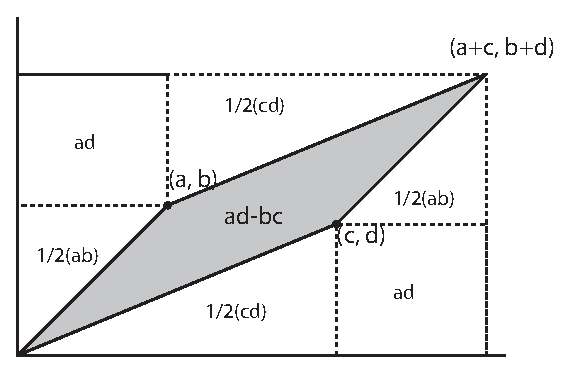
\epsfig{file=parallelogram.eps, scale=.75}
\end{center}

The area of the parallelogram is $$|(a+c)(b+d)-2ad-ab-cd|=|ab+ad+bc+cd-2ad-ab-cd|=|ad-bc|$$

\end{frame}



\begin{frame}
\frametitle{Determinant}

\ \\Now, let's see an example of computing determinant. Say, we have following matrix, $A$. \pause

\begin{eqnarray}
A & = & \begin{pmatrix}
1 & 0 & 3 \\
1 & 2 & -1 \\
2 & 1 & -1
\end{pmatrix} \nonumber
\end{eqnarray} \pause

\ \\Then, the determinant by expanding the first row is:

$$ |A| = 1 \times 
\begin{vmatrix}
2 & -1 \\
1 & -1
\end{vmatrix} - 0 \times
\begin{vmatrix}
1 & -1 \\
2 & -1
\end{vmatrix} + 3 \times
\begin{vmatrix}
1 & 2 \\
2 & 1
\end{vmatrix} $$ \pause

$$ |A| = 1 \times (-1) - 0 \times 1 + 3 \times (-3) = -10$$

\end{frame}



%\begin{frame}
%\frametitle{Determinant} 

%Facts needed to define determinant :

%\begin{defn}
% A \alert{permutation} of the set of integers $\{1, 2, \hdots, J \}$ is an arrangement of these integers in some order without omissions or repetition.
%\end{defn}

%For example, consider $\{1, 2, 3, 4\}$
%\begin{itemize}
%\item[] $\{3, 2, 1 , 4 \}$
%\item[] $\{4, 3, 2, 1 \} $
%\end{itemize}

%If we have $J$ integers then there are $J!$ permutations

%\end{frame}



%\begin{frame}
%\frametitle{Determinant}

%\begin{defn}
%An \alert{inversion} occurs when a larger integer occurs before a smaller integer in a permutation
%\begin{itemize}
%\item[] Even permutation: total inversions are even
%\item[] Odd permutation: total inversions are odd
%\end{itemize}
%\end{defn}

%Count the inversions
%\begin{itemize}
%\item[] $\{3, 2, 1\}$
%\item[] $\{1, 2, 3\}$
%\item[] $\{3, 1, 2\}$
%\item[] $\{2, 1, 3\}$
%\item[] $\{1, 3, 2\}$
%\item[] $\{2, 3, 1\}$
%\end{itemize}

%\end{frame}




%\begin{frame}
%\frametitle{Determinant}

%\begin{defn}
%For a square $n x n$ matrix $A$, we will call an \alert{elementary product} an $n$ element long product, with no two components coming from the same row or column.  We will call a \alert{signed} elementary product one that multiplies odd permutations of the column numbers by $-1$.  
%\end{defn}

%\vspace{1in}

%\pause 

%\only<1-2>{\invisible<1>{$\begin{pmatrix}
%a_{11} & a_{12} \\
%a_{21} & a_{22} \\
%\end{pmatrix}$}}
%\pause 

%\only<3>{$\begin{pmatrix}
%a_{11} & a_{12} & a_{13} \\
%a_{21} & a_{22} & a_{23}\\
%a_{31} & a_{32} & a_{33}\\
%\end{pmatrix}$}

%\only<3>{There are $n!$ elementary products}

%\end{frame}



%\begin{frame}
%\frametitle{Determinant}

%\begin{defn}
%Suppose $A$ is an $n \times n $ matrix.  Define the determinant function $\text{det}(A)$ to be the sum of signed elementary products from $A$.  Call $\text{det}(A)$ the \alert{determinant} of $A$ 
%\end{defn}

%\only<1-4>{\invisible<1>{Suppose $A$ is a $2 \times 2$ matrix} 
%\begin{eqnarray}
%\invisible<1-2>{\text{det}(A) & = & \text{det} \begin{pmatrix} a_{11} & a_{12} \\
%a_{21} & a_{22} \\
%\end{pmatrix}} 
%\nonumber \\
%\invisible<1-3>{& = & a_{11} a_{22} - a_{12} a_{21} \nonumber } 
%\end{eqnarray} 
%}

%\only<5->{
%Suppose $A$ is a $3 \times 3$ matrix.  
%\begin{eqnarray}
%\invisible<1-5>{\text{det}(A) & = & \text{det} \begin{pmatrix}
%a_{11} & a_{12} & a_{13} \\
%a_{21} & a_{22} & a_{23} \\
%a_{31} & a_{32} & a_{33} \\
%\end{pmatrix}} 
%\nonumber \\
%\invisible<1-6>{& = & a_{11} a_{22} a_{33} - a_{11} a_{23} a_{32} - a_{12}a_{21} a_{33} \nonumber \\
%& & + a_{12} a_{23} a_{31} + a_{13} a_{21} a_{32} - a_{13} a_{22} a_{31} \nonumber}
%\end{eqnarray}
%}

%\invisible<1-7>{{\tt R Code!}}

%\pause \pause \pause \pause \pause \pause \pause 

%\end{frame}





\begin{frame}

\begin{itemize}
\item \textcolor{mygray}{Determinant}
\item \textcolor{myblack}{Eigenvalues and Eigenvectors}
\item \textcolor{mygray}{Multivariate Function}
\item \textcolor{mygray}{Multivariate Derivative}
\end{itemize}

\end{frame}



\begin{frame}
\frametitle{An Introduction to Eigenvectors, Values, and Diagonalization}


\begin{defn}
Suppose $\boldsymbol{A}$ is an $N \times N$ matrix and $\lambda$ is a scalar.  \\

If 

\begin{eqnarray}
\boldsymbol{A}\boldsymbol{x} &= & \lambda \boldsymbol{x} \nonumber 
\end{eqnarray}

Then $\boldsymbol{x}$ is an eigenvector and $\lambda$ is the associated eigenvalue

\end{defn}

\pause 

\begin{itemize}
\invisible<1>{\item[-] $\boldsymbol{A}$ stretches the eigenvector $\boldsymbol{x}$ } \pause 
\invisible<1-2>{\item[-] $\boldsymbol{A}$ stretches $\boldsymbol{x}$ by $\lambda$ } \pause 
\invisible<1-3>{\item[-] To find eigenvectors/values: ({\tt eigen} in {\tt R} ) } \pause 
\begin{itemize}
\invisible<1-4>{\item Find $\lambda$ that solves $\text{det}(\boldsymbol{A}- \lambda \boldsymbol{I}) = 0 $} \pause 
\invisible<1-5>{\item Find vectors in null space} of: \pause 
\begin{eqnarray}
\invisible<1-6>{(\boldsymbol{A} - \lambda \boldsymbol{I} ) &= & 0 \nonumber } 
\end{eqnarray}
\end{itemize}
\end{itemize}


\end{frame}



\begin{frame}
\frametitle{An Introduction to Eigenvectors, Values and Diagonalization}

\ \\After we define invertibility, eigenvalues and eigenvectors, a natural question would be: what is the relationship between those concepts. \pause 

\ \\Following theorem gives us the answer.

\end{frame}

\begin{frame}
\frametitle{An Introduction to Eigenvectors, Values, and Diagonalization}

\begin{thm}
Suppose $\boldsymbol{A}$ is an invertible $N \times N$ matrix and further suppose that $\boldsymbol{A}$ has $N$ distinct eigenvalues and $N$ linearly independent eigenvectors.  Then we can write $\boldsymbol{A}$ as, 

\begin{eqnarray}
\boldsymbol{A} &= & \boldsymbol{W}\begin{pmatrix}
\lambda_{1} & 0 & \hdots & 0 \\
0 & \lambda_{2} & \hdots & 0 \\
\vdots & \vdots & \ddots & \vdots \\
0 & 0&  \hdots & \lambda_{N}\\
\end{pmatrix}
\boldsymbol{W}^{-1} \nonumber 
\end{eqnarray}

where $\boldsymbol{W} = \left(\boldsymbol{w}_{1}, \boldsymbol{w}_{2}, \hdots, \boldsymbol{w}_{N} \right)$ is an $N \times N$ matrix with the $N$ eigenvectors as column vectors.  

\end{thm}

\end{frame}


\begin{frame}
Proof:\\

Note
\begin{eqnarray}
\boldsymbol{A}\boldsymbol{W} & = & \begin{pmatrix} \lambda_{1} \boldsymbol{w}_{1} &  \lambda_{2} \boldsymbol{w}_{2}  & \hdots  & \lambda_{N} \boldsymbol{w}_{N} \end{pmatrix} \nonumber \pause \\ 
& = & \boldsymbol{W}\boldsymbol{\Lambda} \nonumber \pause \\
\boldsymbol{A} & = & \boldsymbol{W}\boldsymbol{\Lambda} \boldsymbol{W}^{-1} \nonumber 
\end{eqnarray}

\end{frame}



\begin{frame}
\frametitle{Examples of Diagonalization}

Suppose $\boldsymbol{A}$ is an $N \times N$ invertible matrix with eigenvalues $\boldsymbol{\lambda} = (\lambda_{1}, \lambda_{2}, \hdots, \lambda_{N})$ and eigenvectors $\boldsymbol{W}$.  Calculate $\boldsymbol{A} \boldsymbol{A} = \boldsymbol{A}^{2}$ \pause

\begin{eqnarray}
\boldsymbol{A}\boldsymbol{A} & = & \boldsymbol{W} \boldsymbol{\Lambda} \boldsymbol{W}^{-1} \boldsymbol{W} \boldsymbol{\Lambda} \boldsymbol{W}^{-1} \nonumber \pause \\
& = &  \boldsymbol{W} \begin{pmatrix}
\lambda_{1} & 0 & \hdots & 0 \\
0 & \lambda_{2} & \hdots & 0 \\
\vdots & \vdots & \ddots & \vdots \\
0 & 0&  \hdots & \lambda_{N}\\
\end{pmatrix} \begin{pmatrix}
\lambda_{1} & 0 & \hdots & 0 \\
0 & \lambda_{2} & \hdots & 0 \\
\vdots & \vdots & \ddots & \vdots \\
0 & 0&  \hdots & \lambda_{N}\\
\end{pmatrix} \boldsymbol{W}^{-1} \nonumber \pause \\
& = & \boldsymbol{W} \begin{pmatrix}
\lambda_{1}^{2} & 0 & \hdots & 0 \\
0 & \lambda_{2}^{2} & \hdots & 0 \\
\vdots & \vdots & \ddots & \vdots \\
0 & 0&  \hdots & \lambda_{N}^{2} \\
\end{pmatrix} \boldsymbol{W}^{-1} \nonumber 
\end{eqnarray}


\end{frame}



\begin{frame}

\begin{itemize}
\item \textcolor{mygray}{Determinant}
\item \textcolor{mygray}{Eigenvalues and Eigenvectors}
\item \textcolor{myblack}{Multivariate Function}
\item \textcolor{mygray}{Multivariate Derivative}
\end{itemize}

\end{frame}





\begin{frame}
\frametitle{Multivariate Functions}


\only<1>{\begin{eqnarray}
f(x_{1}, x_{2}) & = & x_{1}  + x_{2} \nonumber 
\end{eqnarray}} 

\only<2>{\begin{eqnarray}
f(x_{1}, x_{2}) & = & x_{1}^2 + x_{2}^2 \nonumber 
\end{eqnarray}}



\only<3>{\begin{eqnarray}
f(x_{1}, x_{2}) & = &   \sin(x_1)\cos(x_2)   \nonumber 
\end{eqnarray}}


\only<4>{\begin{eqnarray}
f(x_{1}, x_{2}) & = &   -(x-5)^2 - (y-2)^2  \nonumber 
\end{eqnarray}}

\only<5>{\begin{eqnarray} 
f(x_{1}, x_{2}, x_{3} ) & = & x_1 + x_2 + x_3 \nonumber 
\end{eqnarray} }

\only<6>{\begin{eqnarray} 
f(\boldsymbol{x} ) & = & f(x_{1}, x_{2}, \hdots, x_{N} ) \nonumber \\
							& = & x_{1} +x_{2} + \hdots + x_{N} \nonumber \\
							& = & \sum_{i=1}^{N} x_{i} \nonumber 
\end{eqnarray} } 							



\end{frame}




\begin{frame}
\frametitle{Multivariate Functions}

\begin{defn}
Suppose $f:R^{n} \rightarrow R^{1}$.  We will call $f$ a multivariate function.  We will commonly write,
\begin{eqnarray}
f(\boldsymbol{x}) & = & f(x_{1}, x_{2}, x_{3}, \hdots, x_{n} ) \nonumber 
\end{eqnarray}

\end{defn}

\begin{itemize}
\item[-] $R^{n} = R \underbrace{\times}_{\text{cartesian}} R \times R \times \hdots R $
\item[-] The function we consider will take $n$ inputs and output a single number (that lives in $R^{1}$, or the real line)
\end{itemize} 

\end{frame}


\begin{frame}
\frametitle{Example 1} 


\only<1>{\begin{eqnarray}
f(x_{1}, x_{2}, x_{3}) & = & x_1  + x_2 + x_3 \nonumber 
\end{eqnarray}
Evaluate at $\boldsymbol{x} = (x_{1}, x_{2}, x_{3}) = (2, 3, 2) $ \\
\begin{eqnarray}
f(2, 3, 2) & = & 2 + 3 + 2 \nonumber \\
			& = & 7 \nonumber 
\end{eqnarray}} 


\only<2>{\begin{eqnarray}
f(x_{1}, x_{2} ) & = & x_{1} + x_{2} + x_{1} x_{2} \nonumber 
\end{eqnarray} 
Evaluate at $\boldsymbol{w} = (w_{1}, w_{2} ) = (1, 2) $ 
\begin{eqnarray}
f(w_{1}, w_{2}) & = & w_{1} + w_{2} + w_{1} w_{2} \nonumber \\
								& = & 1  + 2  + 1 \times 2 \nonumber \\
								& = & 5 \nonumber 
\end{eqnarray}								
}								




\end{frame}



\begin{frame}
\frametitle{Preferences for Multidimensional Policy}

Recall that in the spatial model, we suppose policy and political actors are located in a space.  \pause \\
\invisible<1>{Suppose that policy is $N$ dimensional---or $\boldsymbol{x} \in \Re^{N}$.} \pause \\
\invisible<1-2>{Suppose that legislator $i$'s utility is a $U:\Re^{N} \rightarrow \Re^{1}$ and is given by,} \pause  
\begin{eqnarray}
\invisible<1-3>{U(\boldsymbol{x}) & = & U(x_{1}, x_{2}, \hdots, x_{N} ) \nonumber } \pause \\
\invisible<1-4>{					& = & - (x_{1} - \mu_{1} )^2 - (x_{2} - \mu_{2})^2 - \hdots - (x_{N} - \mu_{N})^{2} \nonumber \\} \pause 
\invisible<1-5>{						& = & -\sum_{j=1}^{N} (x_{j} - \mu_{j} )^{2} \nonumber } \pause 
\end{eqnarray}							

\invisible<1-6>{Suppose $\boldsymbol{\mu} = (\mu_{1}, \mu_{2}, \hdots, \mu_{N} ) = (0, 0, \hdots, 0)$.  } \pause 
\invisible<1-7>{Evaluate legislator's utility for a policy proposal of $\boldsymbol{m} = (1, 1, \hdots, 1)$.  } \pause 
\begin{eqnarray}
\invisible<1-8>{U(\boldsymbol{m} ) & = & U(1, 1, \hdots, 1) \nonumber} \pause  \\
\invisible<1-9>{							  & = & - (1 - 0)^2 - (1- 0) ^2 - \hdots - (1- 0) ^2 } \nonumber \pause \\
\invisible<1-10>{							& = & -\sum_{j=1}^{N} 1}\pause \invisible<1-11>{ = - N }  \nonumber  \\
\end{eqnarray} 


\end{frame}



\begin{frame}

\begin{itemize}
\item \textcolor{mygray}{Determinant}
\item \textcolor{mygray}{Eigenvalues and Eigenvectors}
\item \textcolor{mygray}{Multivariate Function}
\item \textcolor{myblack}{Multivariate Derivative}
\end{itemize}

\end{frame}



\begin{frame}
\frametitle{Multivariate Derivative} 
\begin{defn} 
Suppose $f:X \rightarrow \Re^{1}$, where $X \subset \Re^{n}$. $f(\boldsymbol{x}) = f(x_{1}, x_{2}, \hdots, x_{N} ) $.  If the limit, \\
\small
\begin{eqnarray}
\frac{\partial}{\partial x_{i} } f(\boldsymbol{x}_{0}  ) & = & \frac{\partial}{\partial x_{i} }  f(x_{01}, x_{02}, \hdots,x_{0i}, x_{0i+1}, \hdots,  x_{0N} ) \nonumber \\
& = & \lim_{h\rightarrow 0}  \frac{f(x_{01}, x_{02}, \hdots, x_{0i} + h ,  \hdots x_{0N} ) - f(x_{01}, x_{02} , \hdots,x_{0 i},\hdots,  x_{0N} )} {h}  \nonumber 
\end{eqnarray}

exists then we call this the partial derivative of $f$ with respect to $x_{i}$ at the value $\boldsymbol{x}_{0} = (x_{01}, x_{02}, \hdots, x_{0N})$.

\end{defn}
\end{frame}


\begin{frame}
\frametitle{Rules for Taking Partial Derivatives}

Partial Derivative: $\frac{\partial f(\boldsymbol{x}) }{\partial x_{i} }$ \pause
\begin{itemize}
\item[-] Treat each instance of $x_{i}$ as a variable that we would differentiate before \pause
\item[-] Treat each instance of $\boldsymbol{x}_{-i} = (x_{1}, x_{2} , x_{3} , \hdots, x_{i-1}, x_{i+1}, \hdots, x_{n})$ as a constant
\end{itemize}

\end{frame}


\begin{frame}
\frametitle{Example Partial Derivatives} 


\begin{eqnarray}
f(\boldsymbol{x}) & = & f(x_{1}, x_{2}) \nonumber \\
							& = & x_{1} + x_{2}\nonumber 
\end{eqnarray}							

Partial derivative, with respect to $x_{1}$ at $(x_{01}, x_{02})$
\begin{eqnarray}
\frac{\partial f(x_{1}, x_{2} ) } {\partial x_{1} }|_{(x_{01}, x_{02} )} & = &  1 + 0|_{x_{01}, x_{02}}  \nonumber \\
																	& = & 1 \nonumber 
\end{eqnarray}																	


\end{frame}


\begin{frame}
\frametitle{Example Partial Derivatives}

\begin{eqnarray}
f(\boldsymbol{x}) & = & f(x_{1}, x_{2}, x_{3}) \nonumber \\
							& = & x_{1}^2 \log(x_{1}) + x_{2}x_{1}x_{3} + x_{3}^2 \nonumber 
\end{eqnarray}

\pause 
\invisible<1>{What is the partial derivative with respect to $x_{1}$? }  \invisible<1-2>{$x_{2}$?}  \invisible<1-3>{$x_{3}$?} \invisible<1>{Evaluated at $\boldsymbol{x}_{0} = (x_{01}, x_{02}, x_{03} )$. }

\only<1-2>{\begin{eqnarray}
\invisible<1>{\frac{\partial f(\boldsymbol{x}) }{\partial x_{1} } |_{\boldsymbol{x}_{0} } & = & 2 x_{1} \log(x_{1}) +  x_{1}^{2} \frac{1}{x_{1}} + x_{2} x_{3} |_{\boldsymbol{x}_{0} } \nonumber \\
& = & 2 x_{01} \log(x_{01} ) + x_{01}   + x_{02} x_{03} \nonumber }
\end{eqnarray}
}


\only<3>{\begin{eqnarray}
\frac{\partial f(\boldsymbol{x}) }{\partial x_{2} } |_{\boldsymbol{x}_{0} } & = & x_{1} x_{3} |_{\boldsymbol{x}_{0} } \nonumber \\
& = &  x_{01} x_{03} \nonumber 
\end{eqnarray}
}


\only<4>{\begin{eqnarray}
\frac{\partial f(\boldsymbol{x}) }{\partial x_{3} } |_{\boldsymbol{x}_{0} } & = & x_{1} x_{2} + 2 x_{3} |_{\boldsymbol{x}_{0}} \nonumber \\
& = &  x_{01} x_{02}  + 2 x_{03} \nonumber 
\end{eqnarray}
}



\pause\pause 





\end{frame}




\begin{frame}
\frametitle{Rate of Change, Linear Model}

Suppose we regress Approval$_{i}$ rate for Obama in month $i$ on $\text{Employ}_{i}$ and $\text{Gas}_{i}$.  We obtain the following model:
\begin{eqnarray}
\text{Approval}_{i} & = & 0.8  -0.5 \text{Employ}_{i}  -0.25 \text{Gas}_{i} \nonumber 
\end{eqnarray} \pause

We are modeling Approval$_{i} = f(\text{Employ}_{i}, \text{Gas}_{i} )$.  What is partial derivative with respect to employment?
\begin{eqnarray}
\frac{\partial f(\text{Employ}_{i}, \text{Gas}_{i} ) }{\partial \text{Employ}_{i} } & = & -0.5 \nonumber 
\end{eqnarray}


\end{frame}



\begin{frame}
\frametitle{Gradient} 

\begin{defn} 
Suppose $f:X \rightarrow \Re^{1}$ with $X \subset \Re^{n}$ is a differentiable function.  Define the gradient vector of $f$ at $\boldsymbol{x}_{0}$, $\nabla f(\boldsymbol{x}_{0})$ as, 
\begin{eqnarray}
\nabla f (\boldsymbol{x}_{0})  & = & \left(\frac{\partial f (\boldsymbol{x}_{0}) }{\partial x_{1} }, \frac{\partial f (\boldsymbol{x}_{0}) }{\partial x_{2} }, \frac{\partial f (\boldsymbol{x}_{0}) }{\partial x_{3} }, \hdots, \frac{\partial f (\boldsymbol{x}_{0}) }{\partial x_{n} } \right) \nonumber 
\end{eqnarray}

\end{defn}

\begin{itemize}
\item[-] The gradient points in the direction that the function is increasing in the fastest direction
\item[-] We'll use this to do optimization (both analytic and computational)
\end{itemize}



\end{frame}


\begin{frame}
\frametitle{Example Gradient Calculation}

Suppose 
\begin{eqnarray}
f(\boldsymbol{x} ) & = &  f(x_{1}, x_{2}, \hdots, x_{n}) \nonumber \\
							& = & x_{1}^2 + x_{2}^2 + \hdots + x_{n}^2 \nonumber \\ 
							&= & \sum_{i=1}^{n} x_{i}^{2} \nonumber 
\end{eqnarray}							

Then $\nabla f(\boldsymbol{x}^{*})$ is 
\begin{eqnarray}
\nabla f(\boldsymbol{x}^{*}) & = & \left( 2 x_{1}^{*}, 2 x_{2}^{*}, \hdots, 2 x_{n}^{*} \right) \nonumber 
\end{eqnarray}

So if $\boldsymbol{x}^{*} = (3, 3, \hdots, 3)$ then 
\begin{eqnarray}
\nabla f(\boldsymbol{x}^{*}) & = & (2*3, 2*3, \hdots, 2 *3) \nonumber \\
										& = & (6, 6, \hdots, 6) \nonumber 
\end{eqnarray}





\end{frame}






\begin{frame}
\frametitle{Second Partial Derivative}

\begin{defn}
Suppose $f:X \rightarrow \Re$ where $X \subset \Re^{n}$ and suppose that $\frac{\partial f(x_{1}, x_{2}, \hdots, x_{n})}{\partial x_{i} }$ exists.  Then we define, 
\begin{eqnarray}
\frac{ \partial^{2}  f(\boldsymbol{x}) }{\partial x_{j} \partial x_{i} } & \equiv & \frac{\partial}{\partial x_{j} } \left( \frac{\partial f(\boldsymbol{x})  }{\partial x_{i} }  \right) \nonumber 
\end{eqnarray}

\end{defn}

\begin{itemize}
\item[-] Second derivative could be with respect to $x_{i}$ or with some other variable $x_{j}$
\item[-] Nagging question: does order matter?
\end{itemize}


\end{frame}

\begin{frame}
\frametitle{Second Partial Derivative: Order Doesn't Matter} 

\begin{thm} 
Young's Theorem Let $f: X \rightarrow \Re$ with $X \subset \Re^{n}$ be a twice differentiable function on all of $X$.  Then for any $i$, $j$, at all $\boldsymbol{x}^{*} \in X$, 
\begin{eqnarray}
\frac{\partial^{2} } {\partial x_{i} \partial x_{j} }f(\boldsymbol{x}^{*} ) & = &   \frac{\partial^{2} } {\partial x_{j} \partial x_{i} }f(\boldsymbol{x}^{*} ) \nonumber 
\end{eqnarray}

\end{thm}


\end{frame}

\begin{frame}
\frametitle{Second Order Partial Derivates} 

\begin{eqnarray}
f(\boldsymbol{x}) & = & x_{1}^2 x_{2}^2 \nonumber 
\end{eqnarray}

Then, 
\begin{eqnarray}
\frac{\partial^2}{\partial x_{1} \partial x_{1} } f(\boldsymbol{x}) & = & 2 x_{2}^{2} \nonumber \\
\frac{\partial^2}{\partial x_{1} \partial x_{2} } f(\boldsymbol{x}) & = & 4 x_{1} x_{2} \nonumber \\
\frac{\partial^2}{\partial x_{2} \partial x_{2} } f(\boldsymbol{x}) & = & 2 x_{1}^{2} \nonumber 
\end{eqnarray}


\end{frame}








\begin{frame}
\frametitle{Hessians}


\begin{defn}
Suppose $f:X \rightarrow \Re^{1}$ , $X \subset \Re^{n}$, with $f$ a twice differentiable function.  We will define the Hessian matrix as the matrix of second derivatives at $\boldsymbol{x}^{*} \in X$,
\begin{eqnarray}
\boldsymbol{H}(f)(\boldsymbol{x}^{*} )  & = & \begin{pmatrix} 
		\frac{\partial^{2} f }{\partial x_{1} \partial x_{1} } (\boldsymbol{x}^{*} ) & \frac{\partial^{2} f }{\partial x_{1} \partial x_{2} } (\boldsymbol{x}^{*} ) & \hdots & \frac{\partial^{2} f }{\partial x_{1} \partial x_{n} } (\boldsymbol{x}^{*} ) \\
		\frac{\partial^{2} f }{\partial x_{2} \partial x_{1} } (\boldsymbol{x}^{*} ) & \frac{\partial^{2} f }{\partial x_{2} \partial x_{2} } (\boldsymbol{x}^{*} ) & \hdots & \frac{\partial^{2} f }{\partial x_{2} \partial x_{n} } (\boldsymbol{x}^{*} ) \\
		\vdots & \vdots & \ddots & \vdots \\
		\frac{\partial^{2} f }{\partial x_{n} \partial x_{1} } (\boldsymbol{x}^{*} ) & \frac{\partial^{2} f }{\partial x_{n} \partial x_{2} } (\boldsymbol{x}^{*} ) & \hdots & \frac{\partial^{2} f }{\partial x_{n} \partial x_{n} } (\boldsymbol{x}^{*} ) \\
\end{pmatrix} \nonumber 
\end{eqnarray}

\end{defn}		

\begin{itemize}
\item[-] Hessians are symmetric
\item[-] They describe curvature of a function (think, how bended)
\item[-] Will be the basis for second derivative test for multivariate optimization
\end{itemize}

											

\end{frame}


\begin{frame}
\frametitle{An Example}

\pause 

\invisible<1>{Suppose $f:\Re^{3} \rightarrow \Re$, with } \pause 

\begin{eqnarray}
\invisible<1-2>{f(x_{1}, x_{2}, x_{3} ) & = & x_{1}^{2} x_{2}^2 x_{3}^{2} \nonumber } \pause 
\end{eqnarray}


\begin{eqnarray}
\invisible<1-3>{\nabla f(\boldsymbol{x}) & = & (2 x_{1} x_{2}^{2} x_{3}^{2} , 2 x_{1}^{2} x_{2} x_{3}^{2}, 2 x_{1}^{2} x_{2}^{2}, x_{3}) \nonumber } \pause 
\end{eqnarray}


\invisible<1-4>{\begin{eqnarray}
\boldsymbol{H}(f)(\boldsymbol{x}) & = & 
\begin{pmatrix}
2 x_{2}^{2} x_{3}^2 & 4 x_{1} x_{2} x_{3}^{2} & 4 x_{1} x_{2}^{2} x_{3} \\
4 x_{1} x_{2} x_{3}^{2} & 2 x_{1}^{2} x_{3}^{2} & 4 x_{1}^{2} x_{2} x_{3} \\
4 x_{1} x_{2}^{2} x_{3} & 4 x_{1}^{2} x_{2} x_{3} & 2 x_{1}^{2} x_{2}^{2} \\
\end{pmatrix} \nonumber 
\end{eqnarray}}





\end{frame}


\begin{frame}
\frametitle{Functions with Multidimensional Codomains}


\begin{defn}
Suppose $f:R^{m} \rightarrow R^{n}$.  We will call $f$ a multivariate function.  We will commonly write, 
\begin{eqnarray}
f(\boldsymbol{x} ) & = & \begin{pmatrix} 
f_{1} (\boldsymbol{x} ) \\
f_{2} (\boldsymbol{x} ) \\
\vdots \\
f_{n} (\boldsymbol{x} ) \\
\end{pmatrix} \nonumber 
\end{eqnarray}
 \end{defn}

\end{frame}




\begin{frame}
\frametitle{Example Functions}


\only<1>{Suppose $f:\Re \rightarrow \Re^{2} $, 
\begin{eqnarray}
f(t) & = & (t^2, \sqrt(t) ) \nonumber 
\end{eqnarray}
}
\pause 


\only<2>{\invisible<1>{Suppose $f:\Re^{2} \rightarrow \Re^2$ defined as 
\begin{eqnarray}
f(r, \theta) & = & \begin{pmatrix} 
r \cos \theta \\
r \sin \theta \\
\end{pmatrix}\nonumber 
\end{eqnarray}
}}

\pause 
\only<3>{\invisible<1-2>{
	Suppose we have some policy $\boldsymbol{x} \in \Re^{M} $.  Suppose we have $N$ legislators where legislator $i$ has utility
	\begin{eqnarray}
U_{i}(\boldsymbol{x} )  & = & \sum_{j = 1}^{M} -(x_{j} - \mu_{ij} )^2 \nonumber 
\end{eqnarray}
We can describe the utility of all legislators to the proposal as 
\begin{eqnarray}
f(\boldsymbol{x} ) & = & \begin{pmatrix}
\sum_{j=1}^{M} -(x_{j} - \mu_{1j} )^2 \\
\sum_{j=1}^{M} -(x_{j} - \mu_{2j} )^2 \\
\vdots \\
\sum_{j=1}^{M} -(x_{j} - \mu_{Nj} )^2 \\
\end{pmatrix}
\nonumber
\end{eqnarray}
}
}

\end{frame}

\begin{frame}
\frametitle{Jacobian}

\begin{defn}
Suppose $f:X \rightarrow \Re^{n}$, where $X \subset \Re^{m}$, with $f$ a differentiable function.   Define the Jacobian of $f$ at $\boldsymbol{x}$ as 

\begin{eqnarray}
\boldsymbol{J}(f)(\boldsymbol{x} ) & = & \begin{pmatrix}
\frac{\partial f_{1}}{\partial x_{1} } & \frac{\partial f_{1}}{\partial x_{2} } & \hdots & \frac{\partial f_{1}} {\partial x_{m} } \\
\frac{\partial f_{2}}{\partial x_{1} } & \frac{\partial f_{2}}{\partial x_{2} } & \hdots & \frac{\partial f_{2}} {\partial x_{m} } \\
\vdots & \vdots & \ddots & \vdots \\
\frac{\partial f_{n} } {\partial x_{1} } & \frac{\partial f_{n} } {\partial x_{2} } & \hdots & \frac{\partial f_{n} } {\partial x_{m} } \\
\end{pmatrix} \nonumber 
\end{eqnarray}

\end{defn}

\ \\Remark: The Jacobian matrix is important because if the function f is differentiable at a point x, then the Jacobian matrix defines a linear map $R^{n} \rightarrow R^{m}$, which is the best (pointwise) linear approximation of the function f near the point x. This linear map is thus the generalization of the usual notion of derivative, and is called the derivative or the differential of f at x.

\end{frame}


\begin{frame}
\frametitle{Example of Jacobian}

\begin{eqnarray}
f(r, \theta) & = & \begin{pmatrix} 
r \cos \theta \\
r \sin \theta\\
\end{pmatrix} \nonumber 
\end{eqnarray}

\begin{eqnarray}
\boldsymbol{J}(f)(r, \theta) & = & 
\begin{pmatrix}
\cos \theta & - r \sin \theta  \\
\sin \theta &  r \cos \theta \\
\end{pmatrix} \nonumber 
\end{eqnarray}

\end{frame}


\end{document}
